\documentclass{article}

\usepackage{fancyhdr}
\usepackage{extramarks}
\usepackage{amsmath}
\usepackage{amsthm}
\usepackage{amsfonts}
\usepackage{tikz}
\usepackage[plain]{algorithm}
\usepackage{algpseudocode}
\usepackage{mathtools}
\usepackage{graphicx}
\graphicspath{ {./images/} }

\DeclarePairedDelimiter\abs{\lvert}{\rvert}%
\DeclarePairedDelimiter\norm{\lVert}{\rVert}%

\makeatletter
\let\oldabs\abs
\def\abs{\@ifstar{\oldabs}{\oldabs*}}
%
\let\oldnorm\norm
\def\norm{\@ifstar{\oldnorm}{\oldnorm*}}
\makeatother

\newcommand*{\Value}{\frac{1}{2}x^2}%

\usetikzlibrary{automata,positioning}

%
% Basic Document Settings
%

\topmargin=-0.45in
\evensidemargin=0in
\oddsidemargin=0in
\textwidth=6.5in
\textheight=9.0in
\headsep=0.25in

\linespread{1.1}

\pagestyle{fancy}
\lhead{\hmwkAuthorName}
\chead{\hmwkClass\ (\hmwkClassInstructor\ \hmwkClassTime): \hmwkTitle}
\rhead{\firstxmark}
\lfoot{\lastxmark}
\cfoot{\thepage}

\renewcommand\headrulewidth{0.4pt}
\renewcommand\footrulewidth{0.4pt}

\setlength\parindent{0pt}

%
% Create Problem Sections
%

\newcommand{\enterProblemHeader}[1]{
    \nobreak\extramarks{}{Problem \arabic{#1} continued on next page\ldots}\nobreak{}
    \nobreak\extramarks{Problem \arabic{#1} (continued)}{Problem \arabic{#1} continued on next page\ldots}\nobreak{}
}

\newcommand{\exitProblemHeader}[1]{
    \nobreak\extramarks{Problem \arabic{#1} (continued)}{Problem \arabic{#1} continued on next page\ldots}\nobreak{}
    \stepcounter{#1}
    \nobreak\extramarks{Problem \arabic{#1}}{}\nobreak{}
}

\setcounter{secnumdepth}{0}
\newcounter{partCounter}
\newcounter{homeworkProblemCounter}
\setcounter{homeworkProblemCounter}{1}
\nobreak\extramarks{Problem \arabic{homeworkProblemCounter}}{}\nobreak{}

%
% Homework Problem Environment
%
% This environment takes an optional argument. When given, it will adjust the
% problem counter. This is useful for when the problems given for your
% assignment aren't sequential. See the last 3 problems of this template for an
% example.
%
\newenvironment{homeworkProblem}[1][-1]{
    \ifnum#1>0
        \setcounter{homeworkProblemCounter}{#1}
    \fi
    \section{Problem \arabic{homeworkProblemCounter}}
    \setcounter{partCounter}{1}
    \enterProblemHeader{homeworkProblemCounter}
}{
    \exitProblemHeader{homeworkProblemCounter}
}

%
% Homework Details
%   - Title
%   - Due date
%   - Class
%   - Section/Time
%   - Instructor
%   - Author
%

\newcommand{\hmwkTitle}{Homework\ \#9}
\newcommand{\hmwkDueDate}{March 31, 2020}
\newcommand{\hmwkClass}{Physics 926}
\newcommand{\hmwkClassTime}{}
\newcommand{\hmwkClassInstructor}{Professor Ken Bloom}
\newcommand{\hmwkAuthorName}{\textbf{Robert Tabb}}

%
% Title Page
%

\title{
    \vspace{2in}
    \textmd{\textbf{\hmwkClass:\ \hmwkTitle}}\\
    \normalsize\vspace{0.1in}\small{Due\ on\ \hmwkDueDate\ at 5pm}\\
    \vspace{0.1in}\large{\textit{\hmwkClassInstructor\ \hmwkClassTime}}
    \vspace{3in}
}

\author{\hmwkAuthorName}
\date{}

\renewcommand{\part}[1]{\textbf{\large Part \Alph{partCounter}}\stepcounter{partCounter}\\}

%
% Various Helper Commands
%

% Useful for algorithms
\newcommand{\alg}[1]{\textsc{\bfseries \footnotesize #1}}

% For derivatives
\newcommand{\deriv}[1]{\frac{\mathrm{d}}{\mathrm{d}x} (#1)}

% For partial derivatives
\newcommand{\pderiv}[2]{\frac{\partial}{\partial #1} (#2)}

% Integral dx
\newcommand{\dx}{\mathrm{d}x}

% Alias for the Solution section header
\newcommand{\solution}{\textbf{\large Solution}}

% Probability commands: Expectation, Variance, Covariance, Bias
\newcommand{\E}{\mathrm{E}}
\newcommand{\Var}{\mathrm{Var}}
\newcommand{\Cov}{\mathrm{Cov}}
\newcommand{\Bias}{\mathrm{Bias}}

\begin{document}

\maketitle

\pagebreak

\begin{homeworkProblem}
    Show that in $\pi$$\rightarrow$$\mu$$\nu$ decay, \(\abs{\vec{p}_\mu} = \abs{\vec{p}_\nu} = (m_{\pi}^{2} - m_{\mu}^{2}) / 2m_{\pi}\)
\\
\\
    \textbf{Solution}

    Start by defining the momentum four-vectors for each particle in the center of momentum frame. Note that $\sigma$ is the index while $\mu$, $\nu$, and $\pi$ are the names of the particles. In the CM frame, the momentum of the pion must be zero, so by conservation of momentum, the two outgoing particles must have equal and opposite momentum.
    \\
	\[
		\begin{split}
		P_\pi^\sigma=(m_\pi, \vec{0})
		\\
		P_\mu^\sigma=(E_\mu, \vec{p})
		\\
		P_\nu^\sigma=(E_\nu,-\vec{p})
		\end{split}
	\]

	Due to conservation of four-momentum, we can write:
	\[
		\begin{split}
		P_\pi^\sigma = P_\mu^\sigma + P_\nu^\sigma
		\\
		P_\pi^\sigma - P_\nu^\sigma = P_\mu^\sigma
		\end{split}
	\]
	
	Now we contract each side with itself which we can do since this operation is Lorentz invariant:
	\[
		\begin{split}
		(P_\pi - P_\nu)^\sigma (P_\pi - P_\nu)_\sigma = P_\mu^\sigma P_{\mu,\sigma}
		\\
		P_\pi^2 + P_\nu^2 - 2P_\nu^\sigma P_{\pi,\sigma} = m_\mu^2
		\end{split}
	\]
	Since we are assuming the the neutrino is massless, \(P_\nu^2 = m_\nu^2 = 0\) and \(E_\nu = \abs{\vec{p}}\)
	
	\[
		\begin{split}
		m_\pi^2-2\abs{\vec{p}} m_\pi = m_\mu^2
		\\
		-2\abs{\vec{p}} m_\pi = m_\mu^2 - m_\pi^2
		\\
		\abs{\vec{p}} = \frac{m_\pi^2 - m_\mu^2}{2m_\pi}
		\end{split}
	\]
\end{homeworkProblem}

\pagebreak

\begin{homeworkProblem}
   (H\&M exercise 12.13) Predict the ratio of the K$^{-}$ $\rightarrow$ e$^{-}$ $\bar{\nu}_e$ and K$^{-}$ $\rightarrow$ $\mu^{-}$ $\bar{\nu}_\mu$ decay rates. Given that the lifetime of the K is \(\tau = 1.2 \times 10^{-8} s\) and the K $\rightarrow \mu \nu$ branching ratio is 64\%, estimate the decay constant f$_K$. Comment on your assumptions and your result.
   \\
   \\
   \textbf{Solution}
   \\
   In Halzen and Martin, this calculation is done for the $\pi^-$ decay. This decay looks exactly like what we have here, we just need to follow the procedure outlined from equations (12.45) to (12.54). 
   \\
   \\
   Thus we have:
   \[
	   \begin{split}
	   \Gamma(K^- \rightarrow e^- \bar{\nu}_e) = \frac{G^2}{8\pi}f_k^2m_k m_e^2 (\frac{m_k^2-m_e^2}{m_k^2})^2 \\
	   \Gamma(K^- \rightarrow \mu^- \bar{\nu}_\mu) = \frac{G^2}{8\pi}f_k^2m_k m_\mu^2 (\frac{m_k^2-m_\mu^2}{m_k^2})^2 \\
	   \frac{\Gamma(K^- \rightarrow e^- \bar{\nu}_e)}{\Gamma(K^- \rightarrow \mu^- \bar{\nu}_\mu)} = \frac{\frac{G^2}{8\pi}f_k^2m_k m_e^2 (\frac{m_k^2-m_e^2}{m_k^2})^2}{\frac{G^2}{8\pi}f_k^2m_k m_\mu^2 (\frac{m_k^2-m_\mu^2}{m_k^2})^2} = \frac{m_e^2}{m_\mu^2}(\frac{m_k^2-m_e^2}{m_k^2-m_\mu^2})^2
	   \end{split}
   \]
   Now just plug in the relevant numbers, \(m_k = 493.68 MeV, \quad m_\mu = 105.66 MeV, \quad m_e = 0.51100 MeV\)
   \[
	   \frac{\Gamma(K^- \rightarrow e^- \bar{\nu}_e)}{\Gamma(K^- \rightarrow \mu^- \bar{\nu}_\mu)} =  \frac{0.51100^2}{105.66^2}(\frac{493.68^2-0.51100^2}{493.68^2-105.66^2})^2 = 2.5686 \times 10^{-5}
   \]
   The PDG (http://pdg.lbl.gov/2017/listings/rpp2017-list-K-plus-minus.pdf) gives this value as $2.488 \times 10^{-5}$ which is reasonably close to the value obtained here.
   \\
   \\
   We are given that $\tau=1.2 \times 10^{-8}s$ for the decay of the $K^{-}$, and that the branching ratio is 64\%. Since $\Gamma=\frac{1}{\tau}$ and $\Gamma(K^- \rightarrow \mu^- \bar{\nu}_\mu)$ accounts for 64\% of decays, we can write:
   \[
	   \Gamma_{total}\times64\%=\frac{64\%}{\tau}=\frac{G^2}{8\pi}f_k^2m_k m_\mu^2 (\frac{m_k^2-m_\mu^2}{m_k^2})^2=\frac{0.64}{1.2\times10^{-8}}
   \]
   
   Rearranging we get (I cut back the number of digits for the masses since we are only given two digits of $\tau$.):
   \[
	   \begin{split}
	   f_k&=\sqrt{\frac{8\pi}{G^2}\frac{0.64}{1.2\times10^{-8}}\frac{1}{m_km_\mu^2}(\frac{m_k^2}{m_k^2-m_\mu^2})^2} \\
	   &=\sqrt{\frac{8\pi}{(1.17\times 10^{-5})^2}\frac{0.64}{1.8\times10^{16}}\frac{1}{0.494\times 0.106^2}(\frac{0.494^2}{0.494^2-0.106^2})^2} \\
	   &=0.036 \quad GeV = \quad 36 MeV
	   \end{split}
   \]
   A quick note on units: 
   \[
	   \begin{split}
	   [G]=&GeV^{-2} \\ 
	   [m_i]=&GeV \\
	   [\tau]=&GeV^{-1} \\
	   \end{split}
   \]
   But $\tau$ was given to us in seconds, so it had to be converted to $GeV^{-1}$. (\(1s = 1.519 \times 10^{24}GeV^{-1}\))
   
   
\end{homeworkProblem}

\pagebreak

\begin{homeworkProblem}
	If the weak charged current had had a structure $\gamma^\mu(a+b\gamma^5)$, show that for neutrino-electron scattering:
	\[
		\frac{d\sigma}{d\Omega}=\frac{G^2 s}{32\pi}(A^+ + A^-cos^4(\frac{\theta}{2}))
	\]
	for both $\nu_ee$ and $\bar{\nu}_ee$ scattering. If this were the case, then in contrast to Equation 12.64, we would have $\sigma(\nu_ee)=\sigma(\bar{\nu}_ee)$.
	\\
	\\
	\textbf{Solution}
	\begin{figure}[h]
		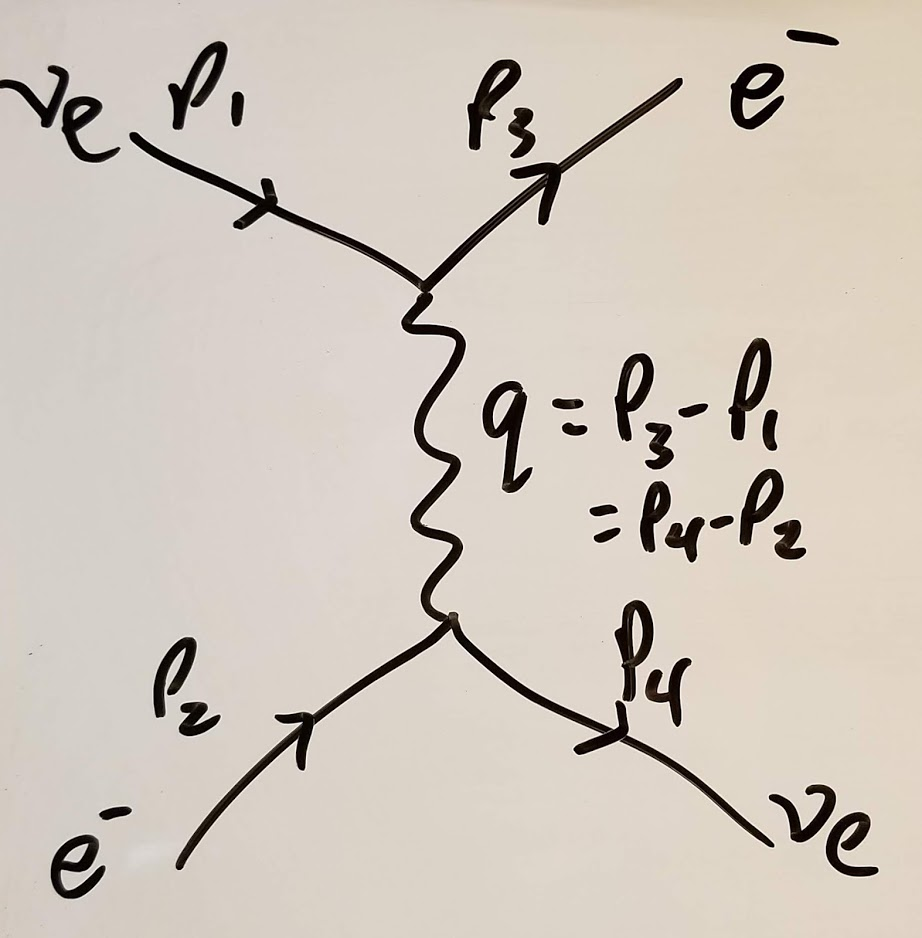
\includegraphics[scale=0.3]{diagram3}
		\centering
		\caption{Feynman diagram for neutrino-electron scattering}
		\label{fullPlot}
		\centering
	\end{figure}
   Start by calculating $\mathcal{M}$
   \[
	   \mathcal{M} = \frac{G}{\sqrt{2}}[\bar{u}(p_4)\gamma^\mu(a+b\gamma^5)u(p_2)][\bar{u}(p_3)\gamma_\mu(a+b\gamma^5)u(p_1)]
   \]
   
\end{homeworkProblem}

\pagebreak

\begin{homeworkProblem}
	Estimate the relative rates for the following decay modes of the $D^0$ meson: \(D^0\rightarrow K^-\pi^+,\pi^-\pi^+,K^+\pi^-\). Compare your estimates to the values given in the PDG.
	\\
	\\
	\textbf{Solution}
    \begin{figure}[h]
    	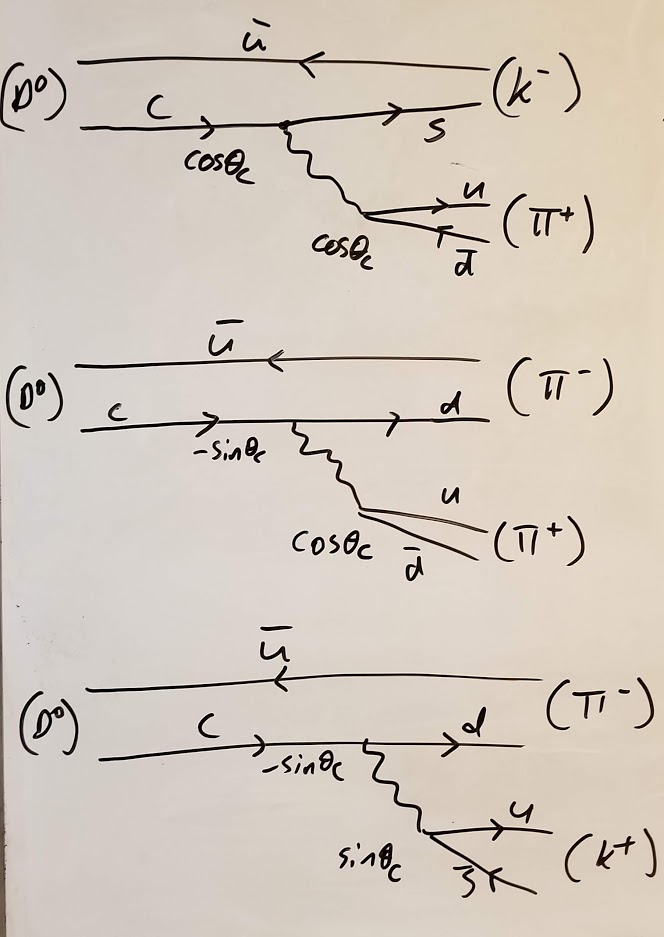
\includegraphics[scale=0.3]{diagram4}
    	\centering
    	\caption{The diagrams for each of the three processes}
    	\label{fullPlot}
    	\centering
    \end{figure}
    To calculate $\mathcal{M}$ for the given diagrams, we must use the Cabibbo angle to find the strengths of the interactions. These can be found on p.281 in Halzen and Martin. What we see from the vertices in these diagrams is:
    \[
	    \begin{split}
	    \abs{\mathcal{M}(D^0\rightarrow K^- \pi^+)}\propto cos^2\theta_c \\
	    \abs{\mathcal{M}(D^0\rightarrow \pi^- \pi^+)}\propto sin\theta_c cos\theta_c \\
	    \abs{\mathcal{M}(D^0\rightarrow \pi^- K^+)}\propto sin^2\theta_c
	    \end{split}
    \]
\end{homeworkProblem}

\pagebreak

\begin{homeworkProblem}
	\textbf{Solution}
    
\end{homeworkProblem}

\pagebreak

\begin{homeworkProblem}
	Because the CKM matrix is unitary, there are constraints among its elements. In particular, the six "dot products" $(row)_i(row)_j^*$ and $(column)_i(column)_j^*$, with $i\neq j$, are all equal to zero. Thus, the six quantities can be expressed graphically in terms of six triangles in the complex plane. These are called unitarity triangles.
	\\
	\\
	\textbf{Part a}
	\\
	Using the Wolfenstein approximation for the CKM matrix that we used in class,
	\[
		V_{CKM}=
		\begin{pmatrix}
		1-\frac{1}{2}\lambda^2 & \lambda & A\lambda^3(\rho-i\eta) \\
		-\lambda & 1-\frac{1}{2}\lambda^2 & A\lambda^2 \\
		A\lambda^3(1-\rho-i\eta) & -A\lambda^2 & 1
		\end{pmatrix}
	\]
	which is good up to factors of $\lambda^4$, to show that four of the six unitarity triangles are squashed. The other two triangles all have sides of the same order of magnitude.
	\\
	\\
	\textbf{Solution}
	\\
	If we let \(A=\rho=\eta=1$ and $\lambda=0.2\), then we can write the CKM matrix as:
	\\
	\[
		V_{CKM}=
		\begin{pmatrix}
		0.98 & 0.2 & 0.008-i0.008 \\
		-0.2 & 0.98 & 0.04 \\
		-i0.008 & -0.04 & 1
	\end{pmatrix}
	\]
	
	We can take the dot product between any row and any other row, $row_i row_j^*$ and the dot product between any column and any other column, $col_i col_j^*$ and these dot products must be equal to zero. This is due to the unitarity of the CKM matrix. Each of these six dot products then represents a triangle in the complex plane whose sides are defined by the points in the complex plane coming from these dot products. 
	\\
	\\
	Here I'll write each product of the six dot products out in the form of a column vector defined like this: \(v=\begin{pmatrix} a_1 \\ a_2 \end{pmatrix}\) where $a_1=$ the real component and $a_2=$ the imaginary component
	\\
	\\
	Triangle 1 ($row_1 row_2^*$):
	\[
		p_1=\begin{pmatrix} -0.2 \\ 0 \end{pmatrix}, \quad 
		p_2=\begin{pmatrix} 0.2 \\ 0 \end{pmatrix}, \quad 
		p_3=\begin{pmatrix} 0.00032 \\ -0.00032 \end{pmatrix}
	\]
	Triangle 2 ($row_1 row_3^*$):
	\[	
		p_1=\begin{pmatrix} 0 \\ -0.008 \end{pmatrix}, \quad 
		p_2=\begin{pmatrix} -0.008 \\ 0 \end{pmatrix}, \quad 
		p_3=\begin{pmatrix} 0.008 \\ -0.008 \end{pmatrix}
	\]
	Triangle 3 ($row_2 row_3^*$):
	\[
		p_1=\begin{pmatrix} 0 \\ 0.0016 \end{pmatrix}, \quad 
		p_2=\begin{pmatrix} -0.04 \\ 0 \end{pmatrix}, \quad 
		p_3=\begin{pmatrix} 0.04 \\ 0 \end{pmatrix}
	\]
	Triangle 4 ($col_1 col_2^*$):
	\[
		p_1=\begin{pmatrix} 0.2 \\ 0 \end{pmatrix}, \quad 
		p_2=\begin{pmatrix} -0.2 \\ 0 \end{pmatrix}, \quad 
		p_3=\begin{pmatrix} 0 \\ 0.0032 \end{pmatrix}
	\]
	Triangle 5 ($col_1 col_3^*$):
	\[
		p_1=\begin{pmatrix} 0.008 \\ -0.008 \end{pmatrix}, \quad 
		p_2=\begin{pmatrix} -0.008 \\ 0 \end{pmatrix}, \quad 
		p_3=\begin{pmatrix} 0 \\ -0.008 \end{pmatrix}
	\]
	Triangle 6 ($col_2 col_3^*$):
	\[
		p_1=\begin{pmatrix} 0.0016 \\ -0.0016 \end{pmatrix}, \quad 
		p_2=\begin{pmatrix} 0.04 \\ 0 	\end{pmatrix}, \quad 
		p_3=\begin{pmatrix} -0.04 \\ 0 \end{pmatrix}
	\]
	
	Each of these triangles is plotted together in the following figures. As you can see in Figure \ref{fullPlot}, most of the triangles are very squished. In the zoom plot in Figure \ref{zoomPlot}, you can see that two of the triangles have sides of comparable length.
		
	\begin{figure}[h]
		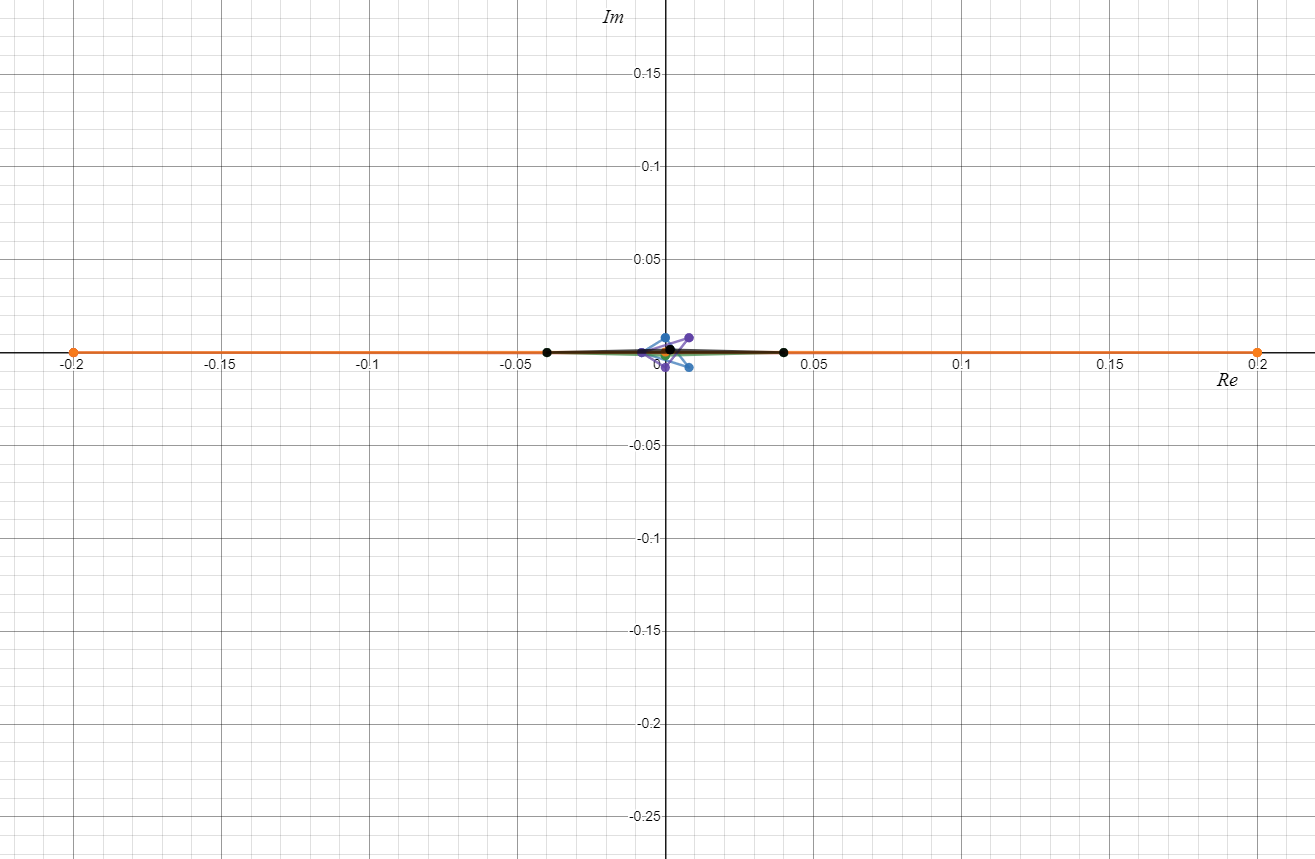
\includegraphics[scale=0.3]{unitaryTriangles}
		\centering
		\caption{The six triangles plotted for $A=\rho=\eta=1$ and $\lambda=0.2$}
		\label{fullPlot}
		\centering
	\end{figure}
	
	
	\begin{figure}[h]			
		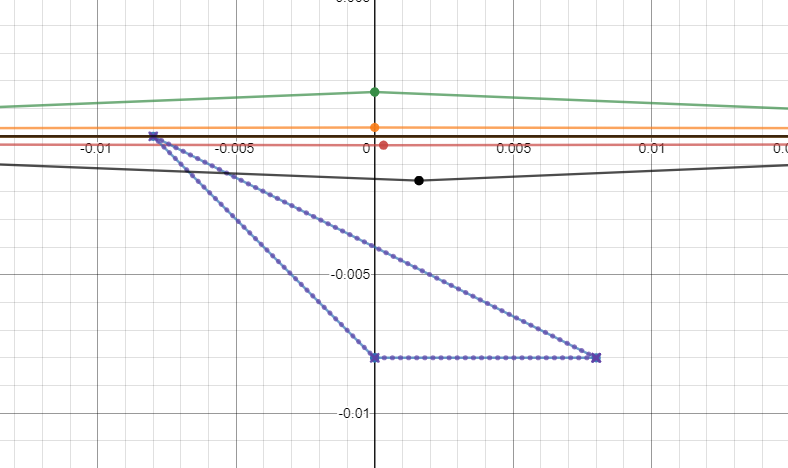
\includegraphics[scale=0.3]{unitaryTrianglesZoom}
		\centering
		\caption{The six triangles plotted to better see the two triangles whose sides are of similar size. The purple triangle is plotted with dotted lines and x's for points so it can be seen overlaid on the other triangle. Since these are plotted using an approximation for the parameters, these look the same but are actually slightly different. (see part b)}
		\label{zoomPlot}
		\centering
	\end{figure}
	
	\textbf{Part b}
	\\
	Show that to leading order in $\lambda$ the two remaining triangles are really the same triangle. 
	\\
	\\
	\textbf{Solution}
	\\
	In part a I immediately wrote all the complex numbers using the numerical approximation for the parameters. Now I will rewrite the complex numbers in vector form for the two triangles which have comparable side lengths. These are triangles 2 and 5
	\\
	\\
	Triangle 2
	\[
		p_1=A\lambda^3(1-\frac{1}{2}\lambda^2)\begin{pmatrix} 1-\rho \\ -\eta \end{pmatrix}, \quad p_2=A\lambda^3\begin{pmatrix} -1 \\ 0 	\end{pmatrix}, \quad 
		p_3=A\lambda^3\begin{pmatrix} \rho \\ -\eta \end{pmatrix}
	\]
	Triangle 5
	\[
		p_1=A\lambda^3(1-\frac{1}{2}\lambda^2)\begin{pmatrix} \rho \\ -\eta \end{pmatrix}, \quad p_2=A\lambda^3\begin{pmatrix} -1 \\ 0 	\end{pmatrix}, \quad 
		p_3=A\lambda^3\begin{pmatrix} 1-\rho \\ -\eta \end{pmatrix}
	\]
		
	To leading order in $\lambda$, which is $\lambda^3$, we can write:
	\\
	\\
	Triangle 2
	\[
		p_1=A\lambda^3\begin{pmatrix} 1-\rho \\ -\eta \end{pmatrix}, \quad 
		p_2=A\lambda^3\begin{pmatrix} -1 \\ 0 	\end{pmatrix}, \quad 
		p_3=A\lambda^3\begin{pmatrix} \rho \\ -\eta \end{pmatrix}
	\]
	Triangle 5
	\[
		p_1=A\lambda^3\begin{pmatrix} \rho \\ -\eta \end{pmatrix}, \quad 
		p_2=A\lambda^3\begin{pmatrix} -1 \\ 0 	\end{pmatrix}, \quad 
		p_3=A\lambda^3\begin{pmatrix} 1-\rho \\ -\eta \end{pmatrix}
	\]
	And now we see that triangles 2 and 5 contain the same points and are the same triangle to leading order in $\lambda$. This is the same result we see in the triangle plots from part a.
	\\
	
	\textbf{Part c}
	\\
	A general representation of the CKM matrix is:
	\[
		\begin{split}
		V_{CKM} = 
		\begin{pmatrix} 
			1 & 0 & 0 \\ 
			0 & c_{23} & s_{23} \\
			0 & -s_{23} & c_{23}\\		
		\end{pmatrix}
		\begin{pmatrix} 
			c_{13} & 0 & s_{13} e^{-i\delta} \\ 
			0 & 1 & 0 \\
			s_{13} e^{i\delta} & 0 & c_{13}\\		
		\end{pmatrix}
		\begin{pmatrix} 
			c_{12} & s_{12} & 0 \\ 
			-s_{12} & c_{12} & 0 \\
			0 & 0 & 1\\		
		\end{pmatrix}
		\\
		=\begin{pmatrix} 
			c_{12}c_{13} & s_{12}c_{13} &  s_{13}e^{-i\delta} \\ 
			-s_{12}c_{23}-c_{12}s_{23}s_{13}e^{i\delta} & c_{12}c_{23}-s_{12}s_{23}s_{13}e^{i\delta} & s_{23}c_{13} \\
			s_{12}s_{23}-c_{12}c_{23}s_{13}e^{i\delta} & -c_{12}s_{23}-s_{12}c_{23}s_{13}e^{i\delta} & c_{23}c_{13}\\		
		\end{pmatrix}
		\end{split}
	\]
	where \(c_{ij} \equiv cos\theta_{ij}\) and \(s_{ij} \equiv sin\theta_{ij}\) and the $\theta_{ij}$ are three rotation angles while $\delta$ is a phase. Show that in this representation the area of each of the six triangles is given by
	\[
		Area= \frac{1}{2}\abs{s_{12}s_{13}s_{23}c_{12}c_{13}^2c_{23}sin\delta}
	\]
	We have six triangles whose sides are defined by points in the complex plane which are found by taking the dot product between rows and columns of the CKM matrix. Given that we have these points, we can easily find the lengths of the sides of the triangle and then apply Heron's Formula to calculate the area from just these side lengths. 
	\\
	\\
	Heron's formula:
	\[
		A=\sqrt{s(s-a)(s-b)(s-c)}
	\]
	Where \(s=\frac{a+b+c}{2}\) and a, b, and c are the lengths of the sides.
	To start, I will choose the triangle defined by taking $row_1 row_2$:
	\\
	\[
		\begin{split}
		P_1 = -s_{12}c_{12}c_{13}c_{23}-s_{13}s_{23}c_{12}^2c_{13}e^{i\delta}\\
			= -s_{12}c_{12}c_{13}c_{23}-s_{13}s_{23}c_{12}^2c_{13}
				\begin{pmatrix} cos\delta \\ sin\delta \end{pmatrix} \\
			= -\begin{pmatrix}
				s_{12}c_{12}c_{13}c_{23}+s_{13}s_{23}c_{12}^2c_{13}cos\delta \\
				s_{13}s_{23}c_{12}^2c_{13}sin\delta
			   \end{pmatrix} \\
		\end{split}		
	\]
	
	\[
		\begin{split}
		P_2 = s_{12}c_{12}c_{13}c_{23}-s_{12}^2s_{13}s_{23}c_{13}e^{i\delta}\\
			= s_{12}c_{12}c_{13}c_{23}-s_{12}^2s_{13}s_{23}c_{13}
				\begin{pmatrix} cos\delta \\ sin\delta \end{pmatrix} \\
			= \begin{pmatrix} 
				s_{12}c_{12}c_{13}c_{23}-s_{12}^2s_{13}s_{23}c_{13}cos\delta \\
				-s_{12}^2s_{13}s_{23}c_{13}sin\delta
				 \end{pmatrix}				
		\end{split}		
	\]
		
	\[
		\begin{split}
			P_3 = s_{13}s_{23}c_{13}e^{-i\delta} \\
			= \begin{pmatrix}
			s_{13}s_{23}c_{13}cos\delta\\
			-s_{13}s_{23}c_{13}sin\delta
			\end{pmatrix}			
		\end{split}		
	\]
	Now to find the lengths of the sides. I will define \(a=\overline{\rm P_1 P}_2\), \(b=\overline{\rm P_1 P}_3\), and \(c=\overline{\rm P_2 P}_3\). Now to calculate the these side lengths:
	\[
		a = \sqrt{(-s_{12}c_{12}c_{13}c_{23}-s_{13}s_{23}c_{12}^2c_{13}cos\delta-s_{12}c_{12}c_{13}c_{23}-s_{12}^2s_{13}s_{23}c_{13}cos\delta)^2+(s_{13}s_{23}c_{12}^2c_{13}sin\delta+s_{12}^2s_{13}s_{23}c_{13}sin\delta)^2}
	\]
	\[
		b = 
		\sqrt{(-s_{12}c_{12}c_{13}c_{23}-s_{13}s_{23}c_{12}^2c_{13}cos\delta-s_{13}s_{23}c_{13}cos\delta)^2+(s_{13}s_{23}c_{12}^2c_{13}sin\delta+s_{13}s_{23}c_{13}sin\delta)^2}
	\]
	\[
		c = 
		\sqrt{(s_{12}c_{12}c_{13}c_{23}-s_{12}^2s_{13}s_{23}c_{13}cos\delta-s_{13}s_{23}c_{13}cos\delta)^2+(-s_{12}^2s_{13}s_{23}c_{13}sin\delta+s_{13}s_{23}c_{13}sin\delta)^2}
	\]
	
\end{homeworkProblem}


\end{document}
